\chapter{Design}
\label{design}
\section{Program Requirements}
\label{programRequirements}

\subsection{Motivation}
While the detriments to SAON technologies are well-known \cite{Akbarzadeh2013}, \cite{Heupel2006}, \cite{Howard2002},  \cite{Kessel2015}, \cite{Steel2014} there few tools/services to analytically design SAONs around them.  Further, none of these tools/services are free and open-source.


\subsubsection{Cost Efficiency}
\label{motivationCost}
In section~\ref{CostAltTech}, we discuss the costs of marine telemetry systems, noting that acoustic telemetry systems produce data at a significantly lower ($\ge$10x cheaper) cost than VHF or GPS/Satellite based technologies.  In order to maintain the cost-efficiency of acoustic technology, at least 10$\%$ of the produced transmissions must be captured by the SAON's receiver array.  Given the numerous (but avoidable) impediments to reception of these acoustic signals (\ref{RulesOfThumb}), the array-design process becomes critical to maintaining the cost-efficiency of SAON technologies.  A free network design tool would help to maintain the cost-efficiency of SAONs by eliminating costs surrounding their design and evaluation.  


\subsubsection{Metrics}
\label{motivationMetrics}
The computation of network metrics (Absoloute Recovery Rate, Unique Recovery Rate, Network Sparsity) is very labor intensive at large scale.  Additionally, the process of computation may vary from experiment to experiment.  An automated tool would solve both issues by providing a fast, simple, repeatable, and well-documented method for computation.  Metrics from such a tool would be useful in directly comparing different network deigns.


\subsubsection{Transparency}
\label{motivationTransparency}
An open-sourced tool/service would make the design process more transparent, permitting peer-review and modification.  This would provide increased confidence in the process, and increased adoption of the tool.  Increased adoption would result in a larger number of efficient SAONs, leading to higher data recovery rates, better data quality, increased return-on-investment, and the ability to better address scientific-research questions.


\subsection{Supported Workflows}
\label{workflows}
\subsubsection{Static Analysis}
\label{staticAnalysis}
As mentioned in section~\ref{motivationMetrics}, a primary motive for this tool was the ability to create a repeatable means of measuring the performance of a SAON.  To this end, the ability to measure an existing network design is important.  Users should be presented with network metrics after specifying bathymetry, receiver locations, network properties, and an animal model for a given study site.


\subsubsection{Optimal Design}
\label{optimalDesign}
The primary motive for this tool is the ability to design optimal SAONs.  Users should be presented with a network design (optimal receiver locations), and network metrics after specifying bathymetry, the number of receivers in the network, network properties, and an animal model for a given study site.


\subsubsection{Optimal Addition}
\label{optimalAddition}
Similar to the problem of optimal design, is the problem of optimal addition: the augmentation of an already existing SAON.  Users should be presented with a network design (optimal augmenting receiver locations), and network metrics after specifying bathymetry, the number of receivers to add to the network, network properties, existing receiver locations, and an animal model for a given study site.

\section{Conceptual Model}
\label{conceptualModel}
\subsection{Time/Space Modeling}
\label{timeSpaceModel}
\subsubsection{Spatial Modeling}
\label{spatialModeling}
To model a 4-dimensional underwater environment (a 3-dimensional spatial grid of various attributes), we use a two-dimensional grid of cells (in the x and y dimensions) containing numerical values.  Numerical values in those cells, combined with other user-defined values, can then be used in various shape functions to generate a third dimension (z) of values for that cell.  In this way, we save significant amounts of memory by computing values for a specific three-dimensional cell on the fly, instead of storing an additional dimension of values.  

\subsubsection{Temporal Modeling}
\label{temporalModeling}
With respect to the passage of time, our model assumes that receivers are stationary throughout the entire experiment.  Furthermore, the animal model does not represent animal movement over time, but the percentage of time an animal would spend in a particular cell over the entire study period.  The animal model therefore represents the tendency of an animal's movements over the expected study period rather than its particular movements in a small time period.  As a result, we need not consider temporally-related phenomena. 




\subsection{Bathymetric Modeling}
\label{bathymetyricModeling}
\subsubsection{Bathymetric Grid}
\label{bathymetricGrid}
Bathymetry files are generally given as two-dimensional matrix of numerical values or a list of x,y,z values.  Bathymetric files describe a three-dimensional space as a regular grid of rectangular prisms (cells) with constant length (x-dimension) and width (y-dimension), but varying negative (depth is negative)  heights (z-dimension).  The resolution of a bathymetric file is given by the x and y (length and width) dimensions of its cells.  For example, a 50 meter Bathymetry file has cell sizes of approximately 50 meters square (although these cells are not necessarily perfectly square).  Bathymetric files list beginning and ending coordinates (North/South Latitudes and East/West Longitudes), as well as the grid size (in rows and columns) in cells.  With these two measurements, one can compute the degrees per cell of latitude and longitude.  Thus, particular latitudes and longitudes can be converted to rows/columns, and back.  

Our program works on a two-dimensional, grid-based system, taking advantage of the grid given by the user-provided bathymetric file.  As stated in section~\ref{spatialModeling}, the bathymetric grid is a grid containing numerical values that describe a third dimension (depth).  The exact spatial extent of this description is given by the bathymetric file.  Thus, the resolution of our program's output is dictated by the resolution of the input bathymetric file. 

\subsubsection{Bathymetric Filetypes}
Two highly popular file formats in Geographical Information Systems are provided by NetCDF and ArcGIS.  NetCDF provides an open source file format that lists a header of metadata and a white-space delimited matrix of numerical values.  ArcGIS is a private institution that supplies many different file types, formats, and encodings for a family of GIS-related software systems.  ArcGIS also supports the encoding and transcription of its proprietary formats to the NetCDF format.  Due to the large number of possible format and encoding combinations in ArcGIS file formats and the ability to translate file these various formats to NetCDF, we natively support the NetCDF standard, and assume that users are capable of converting their data into the NetCDF format.  


\subsubsection{Bathymetric Resolution}
Two key components of our program are the animal model and the bathymetric shadowing model.  These models make decisions based upon the depth at a particular cell and the distance between cells, data which is governed by the input bathymetry file.  As stated in Section~\ref{bathymetricGrid}, the resolution of the program's output is dependant upon the resolution of the input bathymetry file.  Obviously, higher resolution grids will offer higher resolution results; but, high-resolution bathymetric files tend to be difficult to come by.  These files are often held by private agencies, or simply never released to the public.  It may then seem useful to artificially increase the resolution of the simulation by dividing the input file's bathymetric cells into sub-cells of finer resolution, but doing so increases the computational size of the program without meaningfully increasing the accuracy of the results.    
 
 
When subdividing cells, either the sub-cells are given the same depth as their parent cell, or the depth of a sub-cell is interpolated from surrounding cells by some smoothing function.  Subdividing a cell into sub-cells with the same depth makes the assumption that all sub-cells are actually the same depth.  Furthermore, this results in the animal and bathymetric shadowing models making the same depth-based decision for all sub-cells that they would for the larger parent cell, increasing the computational load (see Figure~\ref{duplicate}).  Subdividing a cell into sub-cells with a depth governed by a smoothing function makes the assumption that there are no impeding obstacles between neighboring cells, and that there is a smooth transition between them (see figure~\ref{smooth}).  Subdividing the two cells in Figure~\ref{LoS} half (ignoring for now the y component of our grid) results in the four sub-cells with depths given by a smoothing function (Figure~\ref{smooth}) would result in the large depth change at the sheer cliff face in Figure~\ref{LoS} being smoothed into smaller changes in depth, which would allow the unobstructed transmission of acoustic signals.
\begin{figure}[h!]
	\label{resolutionScale}
	\begin{subfigure}[t]{.4\textwidth}
		\centering
		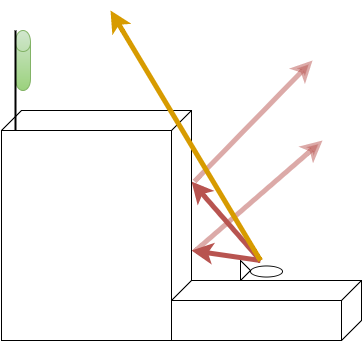
\includegraphics[width=\linewidth]{LoS.png}
		\caption{}\label{LoS}
	\end{subfigure}
	
	\begin{subfigure}[t]{.4\textwidth}
		\centering
		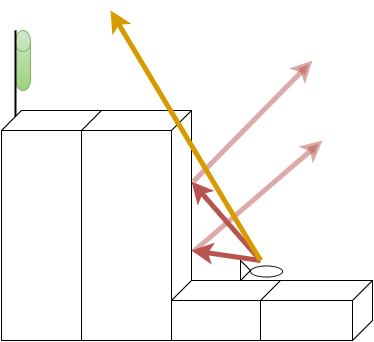
\includegraphics[width=\linewidth]{duplicate.png}
		\caption{}\label{duplicate}
	\end{subfigure}
	
	\begin{subfigure}[t]{.4\textwidth}
		\centering
		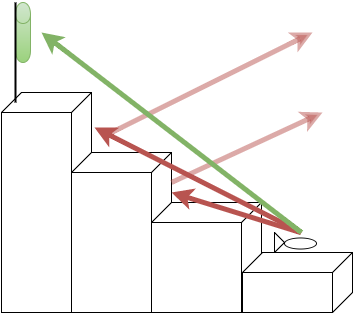
\includegraphics[width=\linewidth]{smooth.png}
		\caption{}\label{smooth}
	\end{subfigure}
	
	\caption{Figure~\ref{LoS} illustrates the bathymetric shadowing model for two adjacent cells within a bathymetric grid.  Figure~\ref{duplicate} shows how artifically increasing the resolution of the bathymetric grid form Figure~\ref{LoS} using the duplication method of cell sub-division does not affect the bathymetric shadowing model.  Figure~\ref{smooth} shows how artificially increasing the resolution using a smoothing function can lead to inflated signal reception.}
\end{figure}

Both strategies (duplicating depth and applying a smoothing function) for artificially increasing the resolution of a bathymetric file disregard the manner in which the bathymetry was originally observed.  Bathymetry is almost always computed as the average observed depth at several points within a geographic area of a given size (resolution).  For example, imagine a particular cell in a bathymetric grid has a steep cliff running across the middle.  Assuming that the sea floor at the top and base of the cliff were perfectly flat, and one measurement was taken at the top of the cliff and one at the bottom, the cell would have a depth equal to the average of the two observed depths.  This average depth would then represent the depth for that entire cell, modeling it as a perfectly flat surface.  Obviously this is problematic as the true nature of the sea floor is misrepresented.  This misrepresentation leads to two conflicting arguments, the first is that the application of smoothing functions or duplicating depths of already averaged data makes faulty assumptions about real-world bathymetry.  On the other hand, because source bathymetric files already represent aggregate data, one could argue that any conclusions drawn from the source bathymetry files are already faulty.  We argue that the conclusions one can make are only as good as the bathymetric information available.  As the resolution of measured bathymetry (bathymetric measurements taken from the real world) increases (becomes finer), so too does the accuracy of the simulation.  While artificially increasing the resolution of a source bathymetric file may skew results, it is sometimes useful for meshing two bathymetric source files of varying resolution into one larger bathymetric dataset.  Our program does not currently support modifying the resolution of source bathymetric files.


\subsubsection{Bathymetric Shadowing}
\label{bathymetricShadowing}
In the real world, the transmission of an acoustic ping originates from the tagged animal and propagates to the receiver.  This propagation is governed by complex interactions with the surrounding environment (including the bottom substrate, water density, distance to the surface/sea-floor, thermoclines, the number of tagged animals in the vicinity, and ambient noise).  Because it is difficult to model these phenomena without significant data on a large number of variables over a large area, our simulation uses a simplified propagation model relying on direct line of sight between a tagged animal and a receiver.  Simply put, in order to receive a transmission, there must exist a physically-unobstructed path between a tagged animal and a receiver.  


\subsection{Animal Modeling}
\label{animalModeling}

\subsubsection{Behavior Grid}
\label{behaviorGrid}
Animals exhibit many different movement patterns and habitat preferences (both of which can vary in three-dimensional space).  This greatly affects their distribution within the study space, and thus the network configuration that should be deployed to capture their movement.  To describe the distribution of transmissions released from tagged animals, we utilize a two dimensional grid of the same dimensions and resolution as the Bathymetry Grid (Section~\ref{bathymetricGrid}).  Each cell in this "Behavior Grid" contains a positive real value indicating, out of all transmissions that will be released over the entire experiment period, the percentage of transmissions that are expected to be released from within that cell's water column.  This value can loosely be though of as the "animal-residency" of a cell since we are effectively measuring the number of animal-hours spent in that cell.  

To populate this 2D grid with values, we provide two behavioral models to simulate the horizontal distribution of animals, and two optional models for the vertical distribution.  Note: we use the terms "animal" and "transmission" interchangeably as we are interested in capturing acoustic transmissions, which are given off by the tags carried by the target species.  


\subsubsection{Animal Movement Modeling}
\label{animalMovementModel}
To simulate tagged animal movement across the two dimensional x/y space (as one would expect to see on a map from above), we provide two basic probabilistic movement models: Random Walk, and Ornstein-Uhlenbeck(OU).  

\paragraph{Random Walk Model}
\label{randomWalkModel}
The Random Walk model assumes that animals move randomly through the environment.  As a result, over the entire study period, each valid grid cell (as defined by the Restricted Vertical Habitat Range (Section~\ref{restrictedVerticalHabitat})) will see an equal amount of animal traffic.  The result is that every valid cell  in the grid will have the same chance of capturing an animal's acoustic transmission.  We assume that tagged individuals will be willing and able to very briefly (in probabilistically negligible time frames) pass through inhospitable (over dry land, through impassible terrain) cells to get to other cells.  This means that disjoint sections of habitat are still equally likely to see animal presence.

\paragraph{Ornstein-Uhlenbeck Model}
\label{ouModel}
The Ornstein-Uhlenbeck(OU) model\cite{OU} supports the idea that over time, animals will tend to congregate near certain points of interest.  This concept models an animal's desire to seek out and remain near a physically significant structure, a region of high food availability, breeding grounds, shelter, etc.  The OU algorithm allows for the modeling of the attraction towards a focal point in the x/y directions separately.  Assuming a center point at the origin of a Cartesian grid, increasing the attraction in the x-direction will bring the distribution closer to the x-axis, and decreasing it will spread the distribution away from the x-axis.  A correlation value ($-1\le x \le 1$) allows for tilting the angle of the distribution.  A positive correlation value tilts the distribution clockwise, and a negative correlation value tilts it counter clockwise.  Correlations of 0 (no tilt), 1 ($180^{\circ}$ tilt), and -1 (-$180^{\circ}$ tilt) will have no observable effect on the distribution.
\begin{figure}[b]
	\label{OUimg}
	\centering
	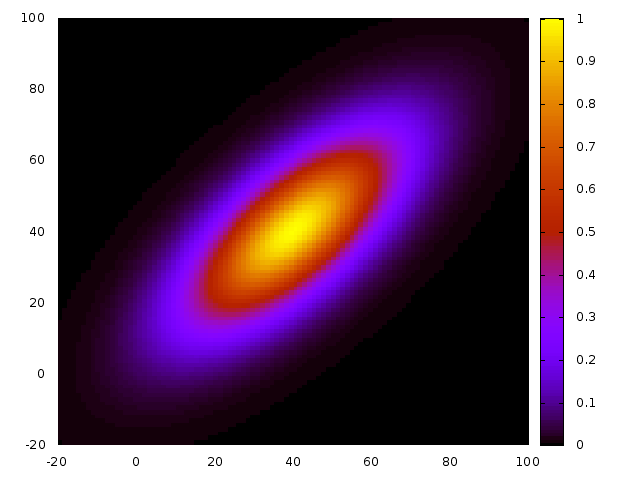
\includegraphics[scale=0.5]{OUpos7.png}
	\caption{}\label{ouimg}
	\caption{An example of a distribution given by the Ornstein-Uhlenbeck Model with a high attraction value in the x-direction, a low attraction value in the y-direction, and a correlation value of 0.7.}
\end{figure}


\subsubsection{Habitat Preference}
\label{habitatPref}
Some animals exhibit the preference to reside within a specific section of the water column; for example, prey animals may prefer hiding in reef heads at the bottom of the water column, while predators will prefer to hover several meters off the bottom.  This preference can be incorporated into the animal model by specifying mean (preferred Depth") and standard deviation("SD of Preferred Depth") values.  These values are given as a measure of the distance (in meters) from the bottom.  For example, specifying a depth of '0' for Preferred Depth indicates that the animal prefers to live on the sea floor, while a value of '5' indicates that the animal prefers to live 5m off the sea floor.  Allowing a standard deviation value allows for the modeling of animals that tend to be sedentary within the water column (a small deviation), and those that migrate through the water column (a large deviation).  Currently, the simulation does not support the modeling of sub-surface animals, and any part of the distribution curve falling below the sea floor will be redistributed along the rest of the curve. 


\subsubsection{Restricted Vertical Habitat Range}
\label{restrictedVerticalHabitat}
Some animals will live only in a specific depth range.  For example, a deep sea fish may live only in depths of 300-400 meters.  To incorporate this into the behavioral model, users can specify a minimum and maximum vertical habitat range for their animal.  If this option is selected, the program will only simulate animals in cells whose maximum depths are between the given minimum and maximum depths.  As in the Random Walk Model, we assume that animals are willing and able to move between disjoint areas of habitat.


\subsection{Receiver Modeling}
\label{receiverModel}

\subsubsection{Acoustic Attenuation}
\label{acousticAttenuation}
As acoustic transmissions travel away from their point of origin, they experience significant attenuation.  We model this attenuation of acoustic signal as a deteriorating function following a Gaussian distribution.  Given a particular distance between a tag and receiver, this distribution describes the probability of capturing the transmission.  Depending upon the environment, the highest probability of detection generally occurs a few meters away from the receiver.

\subsubsection{Detection Range}
\label{detectionRange}
The distance at which a transmission from an acoustic tag can be captured is largely determined by the transmission power of the acoustic tag.  In our model, we assume that all animals have the same model of acoustic tag, and that "transmission range" is instead a property of the receiver referred to as "detection range" ($D_{range}$).  We define the detection range of a receiver to be the average distance (specific to the given study site) at which the probability of detection drops to 5\%.

\subsubsection{Detection Area}
We define the Detection Area of a receiver to be the square plane of grid cells around a receiver which will be considered when evaluating a potential receiver emplacement.  Theoretically, the Detection Area of a receiver is a circle with a radius equal to the receiver's detection range ($D_{range}$).  Within our program, we model the Detection Area as a square grid of cells with an edge length equal to 2*$D_{range}$ + 1, centered on the cell where a receiver will theoretically be placed.  The additional cell ensures odd dimensions for the square, so that there exists a central cell to model as the receiver.  We model a square instead of a circle for simplicity of book keeping (we simply keep track of the detection range, and starting row/column indexes).  The theoretical Detection Range can then be imagined as a circle circumscribed in the square of our model.  At first glance, it might seem that this simplification would alter the probabilistic distribution models as additional "gray" cells (those outside the circle but within the square) are being considered.  However, this is not the case as those models utilize exponential functions based on the absolute distance from the receiver.  Gray cells will therefore contribute exponentially less to the total probability than those cells within the detection range, and their effect on the final probability will be negligible.  

\subsubsection{Network Specification}
There are three distinct ways to place receivers into the model: user specification, optimal placement, and optimal projection.  User Specified Receivers (USR) represent receivers that are already deployed at the study site and are being integrated into a larger network.    Program Placed Receivers are receivers that will be  optimally placed by the program, taking into account existing (user specified) receivers placements using the suppression dynamic explained in section~\ref{suppression}.  Projected Sensors are PPSs that do not count towards the network statistic rates returned by the program.  Instead, their contributed recovery rates are given separately, and represent the marginal benefits of incrementally placing more receivers.  


\section{Evaluation Algorithms}
\label{evaluationAlgorithms}

\subsection{Evaluation of Receiver Emplacements} TODO needs work
\label{evaluationOfReceiver}
Section~\ref{animalModeling} discusses the models used to simulate animal movement.  The animal movement models provide the "Behavior Grid", a 2D grid (of the same size as the specified bathymetry grid) which gives the distribution of animals across the study area, and a shape function which describes a normal distribution of animals within the water column at various depths.  Section~\ref{LoS} discusses the Line of Sight (LoS) model used to simulate the obstruction of acoustic transmission.  Section\ref{receiverModel} discusses how attenuation affects the propagation of acoustic signals and thus the probability of detecting ($P_{range}$) acoustic transmissions from a distance.

\subsection{Evaluation Algorithms (Bias)}
The Evaluation or “Goodness” algorithm is the driving force behind the evaluation of sensor placements.  Given a particular cell at row i and column j, an Evaluation Algorithm will compute a non-negative, rational value representing how well cell (i,j) conforms to that Algorithm's definition of "good".  These values are computed for all cells within the Bathymetry Grid, and stored in the Goodness Grid, a 2D grid of identical size and resolution as the Bathymetry and Behavior Grids.  Thus, $G_{i,j}$ refers to the goodness value of the cell at row i, column j on the bathymetry grid.  

While users are able to write their own “Goodness” algorithms, three basic algorithms are provided.  All Evaluation Algorithms compute the goodness of a potential receiver location ($G_{i,j}$) by summing the number of Estimated Receivable Transmissions (ERT) from all cells within Detection Range of $G_{i,j}$.  The various options each compute ERT differently.

\subsubsection{Animal Only (Option “1”)}
This option prefers to place sensors in areas of high animal activity, completely oblivious to the surrounding bathymetry.  This is useful for when no bathymetric information is available or when animal activity occurs well above the sea floor.   The "Animal Only" option computes ERT for a cell as the animal-residency of a cell (according to the Behavior Grid), multiplied by the probability of detection due to attenuation for that cell's distance from the receiver.


\subsubsection{Visible Fish (Option “3”)}
This option chooses sensor locations that have the best view of areas of high animal activity.  Both animal presence and visibility due to topography are considered. TODO


\subsubsection{Topography Only (Option “2”)}
This option places sensors in areas that have the best visibility of the surrounding area, regardless of the expected animal-residency.  This is useful for experiments where animal habitat is unknown or to be determined.  Here, ERT is computed as the number of observable transmissions from a uniformly distributed animal model.  While this algorithm is referred to as "Topography Only", we implement this by using the "Visible Fish" algorithm with a simplified animal model.  Specifically, we assume that animals are uniformly distributed throughout the environment.  Because animals are uniformly distributed, the more volume a receiver can see, the more transmissions it will receive.  Thus, the algorithm will value cells with the best possible view of the surrounding water columns.



\subsection{Computational Complexity}
\label{computationalComplexity}
A naive solution might be to determine whether or not each cell in the three-dimensional grid can see the receiver.  Given that the volume of a sphere is $\frac{4/3}\pi r^{3}$, this solution would need to consider O($r^{3}$) cells.  Recall however, that we are using a 2-dimensional grid as the basis of our simulation and computing the third dimension as necessary by using a shape function.  Therefore, it is much more computationally efficient to determine the deepest depth in each cell that can be seen by the receiver, and then use integration to compute the probability of detecting transmissions within the water column above that cell ($P_{d}$) .  This leads us to the problem of finding the greatest depth (in each 2D cell) which is visible from the receiver.  We quickly compute this via incremental ray tracing which can be done in O(1) time for O($r^{2}$) cells \cite{Akbarzadeh2013}.   Then, using integration over the shape function, and known min/max depths, the total ($P_{d}$) can be computed in O($r^{2}$) time.  Finally, we determine an average($P_{d}$)  over all O($r^{2}$) cells within detection range.  This metric is used to evaluate each cell within the study area as a candidate for receiver placement.  Thus, our method for evaluating a 3D space can be done in  O($r^{2}$ + $r^{2}$ + $r^{2}$) = O($r^{2}$) time.  One notable difference between our method and the naive method is that the naive method computes the sum probability of detection for each cell in the 3D space, where our method simply integrates to find the probability of detection for the entire a column of water.  


\begin{figure}[t]
	\label{rayTracing}
	\centering
	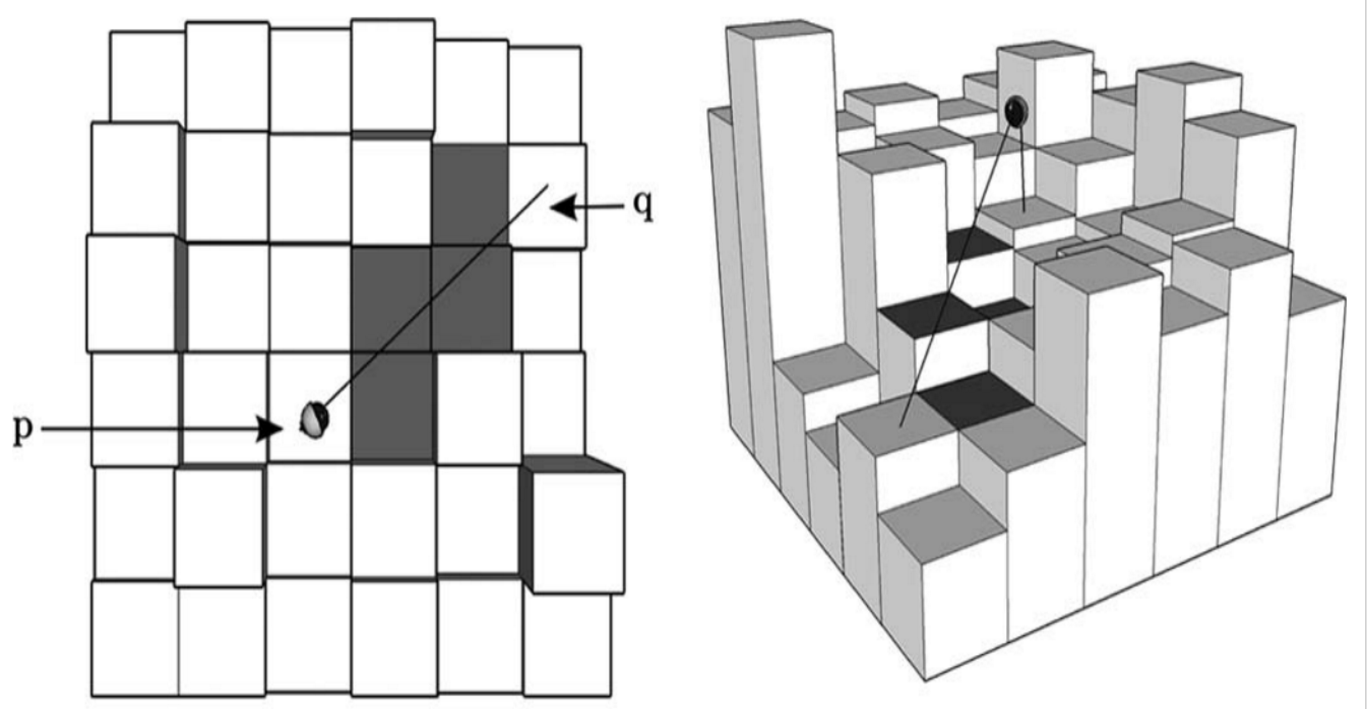
\includegraphics[scale=0.3]{rayTracing.png}
	\caption{An illustration of how ray tracing works within a 3D environment. \cite{Akbarzadeh2013}}
\end{figure}

\begin{figure}[t]
	\label{observableAnimals}
	\centering
	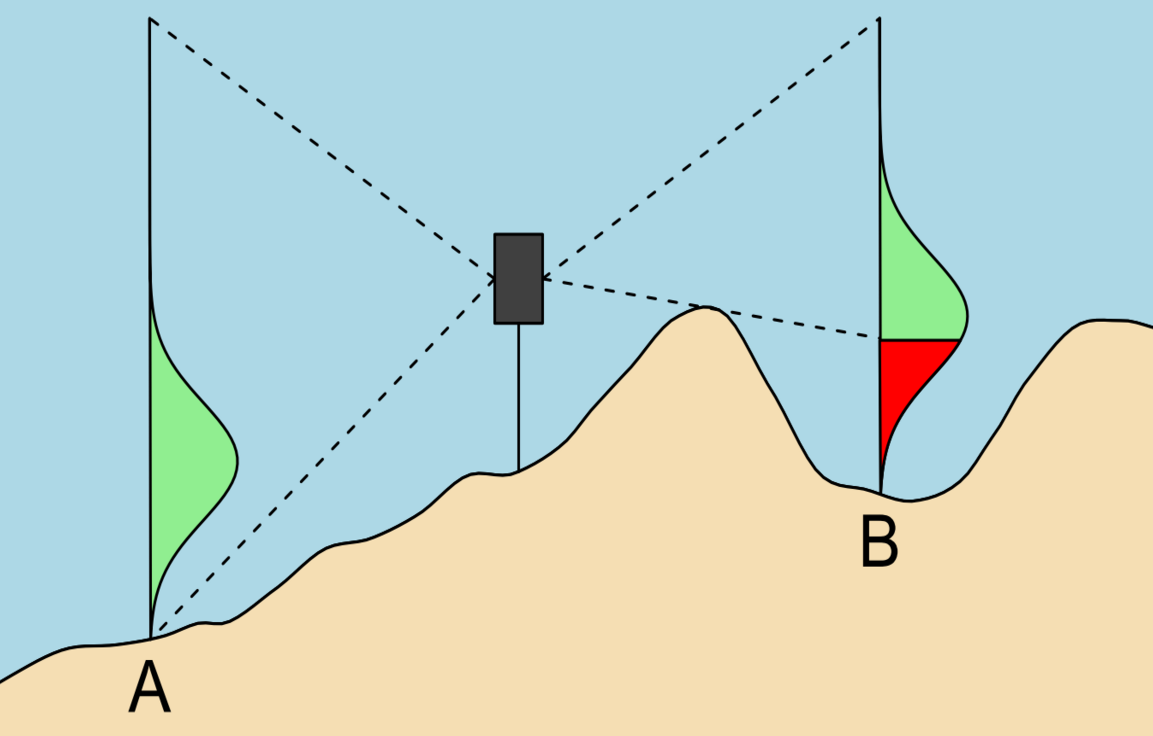
\includegraphics[scale=0.3]{ObservableAnimals.png}
	\caption{An illustration of how ray tracing and integration over a shape function can be used to compute the probability of detecting fish within a cell.  Dotted lines indicate the maximum and minimum depths visible to the receiver.  The normal distributions in green/red indicate the distribution of fish within a given cell as determined by a shape function.  The green portion of the distribution indicates the portion of the distribution that is observable by the receiver and the red indicates the portion that is unobservable by the receiver.  The observable distribution (green) is computed by integration over the shape function.}
\end{figure}


\subsection{Selection of Optimal Emplacements}
\label{selectionOfOptimalEmplacements}
Section~\ref{evaluatingSensorEmplacements} describes the evaluation of cells as potential receiver locations.  The Optimal Design and Optimal Addition work flows (section~\ref{workflows}) require the identification and selection of a user-specified number of receiver emplacements.  Once all cells within the area of interest have been evaluated, the program simply selects the highest rated cells.  The program first selects the user-specified number of optimal receiver locations, and then the number of specified projected receivers.


\section{Suppression}
\label{suppression}
As previously mentioned, the optimality of a network depends greatly upon the way in which data quality is defined.  Some users will want to design a network that covers as much of a study area as possible, while others might want to heavily saturate a small area with sensors to facilitate higher resolution data.  Others may wish to find the receiver locations that return the highest number of unique data points.  Also previously mentioned was the metric of Unique Data Recovery Rate (UDRR) and Absoloute Data Recovery Rate (ADRR) [Section~\ref{dataRecoveryRate}].  For studies which wish to maximize their UDRR, we provide an optional suppression mechanic, which promotes the selection of receiver placements that have a high number of unobserved transmissions.

\subsection{Suppression Area}
As an input to the program, users can specify a Suppression Range Factor as a positive real number.  This factor is used to scale the Detection Range (Section~\ref{detection Range}) and define a grid similar to the Detection Area (Section~\ref{detectionArea}).  The resulting grid is referred to as the Suppression Area.  The Suppression Area is centered over a receiver placement and cells within this area have their number of undetected transmissions reduced according to a Suppression Algorithm.  The suppression mechanic is used during the selection phase of the program.  After selecting each optimal receiver location (Section~\ref{selectionOfOptimalEmplacements}), the Suppression Area around that receiver location is suppressed.  This means that emplacement selection is a sequential process, where selecting each emplacement depends upon the previous selection.  

\subsection{Suppression Algorithms}
\label{suppressionAlgorithms}
To promote the flexibility of our program, we provide users two algorithms for suppression.  The first offers a lower computation time at the cost of divergence from our theoretical model.  The second offers a higher fidelity model, but requires significantly more computation.

\subsubsection{Static Suppression}
\label{staticSuppression}
The Static Suppression algorithm takes a "cookie-cutter" approach and reduces the number of undetected transmissions in the Suppression Area by a user-specified factor.  All cells within the Suppression Area are multiplied by a user-specified value.  This computation is very simplistic, requiring only a scalar multiplication, and as such runs very quickly.  This is useful for simulations that intend to place a very large number of receivers.  The cost of this speed is that the algorithm ignores the attenuation and line of sight models completely.  For instance, a cell that is very far away from the receiver, and whose line of sight to the receiver is obstructed will be reduced by the same factor as a cell with unobstructed line of sight, near the receiver.  Obviously this is not a faithful representation of the conceptual models discussed earlier, but supplied for the sake of convenience.

\subsubsection{Exact Suppression}
\label{exactSuppression}
Let $C_{i,j}$ denote the cell at the $i^{th}$ row and $j^{th}$ column of the 
The Exact Suppression algorithm follows the conceptual model very closely, utilizing the attenuation, and line of sight models via the "Visible Fish" evaluation algorithm (Section~\ref{evaluationAlgorithms}, Bias 3).  The primary purpose of this algorithm was to discount exactly those transmissions which are likely to be observed by a placed receiver.  This algorithm utilizes Algorithm 3, "Visible Fish", to compute the ERT for each cell $C_{i,j}$ within the Suppression Area of the placed receiver $L$.  Then, each cell in the Behavior Grid, $B_{i,j}$  that corresponds to 

Add new receivers (with optimal placement) to an already existing network
Analyze the data recovery rate for a receiver network
Create an optimal receiver network
TODO

\section{Optimal Sensor Projection}
In normal research situations, users will have a set number of receivers to place within their study site.  The process of arriving at this number is likely unscientific, perhaps relying on user estimate (such as the user-perceived feasibility of receiving a given number of receivers).  Rather than guessing at the number of receivers to use, and hoping for an adequate data recovery rate, users should be able to calculate the marginal benefit (additional detections, increased Data Recovery Rates) of utilizing a variable number of receivers.   To this end, the program allows for the projected incremental benefit for a given number of additional receivers.  Our program facilitates this by allowing users to specify a number of receivers to project, returning graphs and metrics of the marginal increase in Data Recovery Rate.  Armed with this data, users can determine an appropriate number of receivers to purchase, or construct an argument for purchasing more receivers.



